%%%%%%%%%%%%%%
%% Run LaTeX on this file several times to get Table of Contents,
%% cross-references, and citations.

%% If you have font problems, you may edit the w-bookps.sty file
%% to customize the font names to match those on your system.

%% w-bksamp.tex. Current Version: Feb 16, 2012
%%%%%%%%%%%%%%%%%%%%%%%%%%%%%%%%%%%%%%%%%%%%%%%%%%%%%%%%%%%%%%%%
%
%  Sample file for
%  Wiley Book Style, Design No.: SD 001B, 7x10
%  Wiley Book Style, Design No.: SD 004B, 6x9
%
%
%  Prepared by Amy Hendrickson, TeXnology Inc.
%  http://www.texnology.com
%%%%%%%%%%%%%%%%%%%%%%%%%%%%%%%%%%%%%%%%%%%%%%%%%%%%%%%%%%%%%%%%

%%%%%%%%%%%%%
% 7x10
%\documentclass{wileySev}

% 6x9
\documentclass{wileySix}

\usepackage{graphicx}
\usepackage{listings}

\usepackage{color}

\definecolor{codegreen}{rgb}{0,0.6,0}
\definecolor{codegray}{rgb}{0.5,0.5,0.5}
\definecolor{codepurple}{rgb}{0.58,0,0.82}
\definecolor{backcolour}{rgb}{0.95,0.95,0.92}

\lstdefinestyle{mystyle}{
    backgroundcolor=\color{backcolour},
    commentstyle=\color{codegreen},
    keywordstyle=\color{magenta},
    numberstyle=\tiny\color{codegray},
    stringstyle=\color{codepurple},
    basicstyle=\footnotesize,
    breakatwhitespace=false,
    breaklines=true,
    captionpos=b,
    keepspaces=true,
    numbers=left,
    numbersep=5pt,
    showspaces=false,
    showstringspaces=false,
    showtabs=false,
    tabsize=2,
    language=sh
}

\lstset{style=mystyle}

%%%%%%%
%% for times math: However, this package disables bold math (!)
%% \mathbf{x} will still work, but you will not have bold math
%% in section heads or chapter titles. If you don't use math
%% in those environments, mathptmx might be a good choice.

% \usepackage{mathptmx}

% For PostScript text
\usepackage{w-bookps}

%%%%%%%%%%%%%%%%%%%%%%%%%%%%%%%%%%%%%%%%%%%%%%%%%%%%%%%%%%%%%%%%
%% Other packages you might want to use:

% for chapter bibliography made with BibTeX
% \usepackage{chapterbib}

% for multiple indices
% \usepackage{multind}

% for answers to problems
% \usepackage{answers}

%%%%%%%%%%%%%%%%%%%%%%%%%%%%%%
%% Change options here if you want:
%%
%% How many levels of section head would you like numbered?
%% 0= no section numbers, 1= section, 2= subsection, 3= subsubsection
%%==>>
\setcounter{secnumdepth}{3}

%% How many levels of section head would you like to appear in the
%% Table of Contents?
%% 0= chapter titles, 1= section titles, 2= subsection titles,
%% 3= subsubsection titles.
%%==>>
\setcounter{tocdepth}{2}

%% Cropmarks? good for final page makeup
%% \docropmarks

%%%%%%%%%%%%%%%%%%%%%%%%%%%%%%
%
% DRAFT
%
% Uncomment to get double spacing between lines, current date and time
% printed at bottom of page.
% \draft
% (If you want to keep tables from becoming double spaced also uncomment
% this):
% \renewcommand{\arraystretch}{0.6}
%%%%%%%%%%%%%%%%%%%%%%%%%%%%%%

%%%%%%% Demo of section head containing sample macro:
%% To get a macro to expand correctly in a section head, with upper and
%% lower case math, put the definition and set the box
%% before \begin{document}, so that when it appears in the
%% table of contents it will also work:

\newcommand{\VT}[1]{\ensuremath{{V_{T#1}}}}

%% use a box to expand the macro before we put it into the section head:

\newbox\sectsavebox
\setbox\sectsavebox=\hbox{\boldmath\VT{xyz}}

%%%%%%%%%%%%%%%%% End Demo


\begin{document}


\booktitle{Internet of Things}
\subtitle{Dalam 24 Jam}

\authors{Rolly M. Awangga\\
\affil{Informatics Research Center}
%Floyd J. Fowler, Jr.\\
%\affil{University of New Mexico}
}

\offprintinfo{Internet of Things, First Edition}{Rolly M. Awangga}

%% Can use \\ if title, and edition are too wide, ie,
%% \offprintinfo{Survey Methodology,\\ Second Edition}{Robert M. Groves}

%%%%%%%%%%%%%%%%%%%%%%%%%%%%%%
%%
\halftitlepage

\titlepage


\begin{copyrightpage}{2019}
%Survey Methodology / Robert M. Groves . . . [et al.].
%\       p. cm.---(Wiley series in survey methodology)
%\    ``Wiley-Interscience."
%\    Includes bibliographical references and index.
%\    ISBN 0-471-48348-6 (pbk.)
%\    1. Surveys---Methodology.  2. Social 
%\  sciences---Research---Statistical methods.  I. Groves, Robert M.  II. %
%Series.\\
%
%HA31.2.S873 2007
%001.4'33---dc22                                             2004044064
\end{copyrightpage}

\dedication{`Jika Kamu tidak dapat menahan lelahnya belajar,
Maka kamu harus sanggup menahan perihnya Kebodohan.'
~Imam Syafi'i~}

\begin{contributors}
\name{Rolly Maulana Awangga,} Informatics Research Center., Politeknik Pos Indonesia, Bandung,
Indonesia



\end{contributors}

\contentsinbrief
\tableofcontents
\listoffigures
\listoftables
\lstlistoflistings


\begin{foreword}
Sepatah kata dari Kaprodi, Kabag Kemahasiswaan dan Mahasiswa
\end{foreword}

\begin{preface}
Buku ini diciptakan bagi yang awam dengan git sekalipun.

\prefaceauthor{R. M. Awangga}
\where{Bandung, Jawa Barat\\
Februari, 2019}
\end{preface}


\begin{acknowledgments}
Terima kasih atas semua masukan dari para mahasiswa agar bisa membuat buku ini 
lebih baik dan lebih mudah dimengerti.

Terima kasih ini juga ditujukan khusus untuk team IRC yang 
telah fokus untuk belajar dan memahami bagaimana buku ini mendampingi proses 
Intership.
\authorinitials{R. M. A.}
\end{acknowledgments}

\begin{acronyms}
\acro{IoT}{Internet Of Things.}

\acro{TCP/IP}{Atomic Energy Commission Transmission Control Protocol atau Internet Protocol.}

\acro{UDP}{User Datagram Protocol.}

\acro{RTP}{Real Time Protocol.}

\acro{FTP}{File Transfer Protocol.}

\acro{HTTP}{Hyper Text Transfer Protocol.}

\acro{DHCP}{Dynamic Host Configuration Protocol.}

\acro{DNS}{Domain Name System.}

\acro{ICMP}{Internet Control Message Protocol.}

\acro{IMAP}{Internet Message Access Protocol.}

\acro{HTTPS}{Hyper Text Transfer Protocol Secure.}

\acro{SSH}{Sucure Shell.}

\acro{SSL}{Secure Socket Layer.}

\acro{IDE}{Integrated Development Environment.}

\acro{LED}{Light Emitting Diode.}
\end{acronyms}

\begin{glossary}
\term{IoT}Merupakan sebuah konektifitas internet yanag dapat bertukar informasi satu sama lainnya dengan benda-benda yang ada disekeliling dengan melalui sensor atau radio frequency identification.

\term{Arduino}Arduino adalah sebuah rangkaian alat elektronik yang memiliki sebuah komponen utama chip mikrokontroler yang dapat di prongram di komputer untuk dapat di kendalikan.

\term{Internet}Merupakan jaringan komputer yang dimana satu jaringan dengan yang lain saling terhubung untuk keperluan komunikasi dan informasi atau dapat disimpulkan internet dapat menghubungkan suatu media elektronik dengan media lainya.

\term{Protokol}adalah suatu aturan yang dapat mengatur sebuah komunikasi untuk menghubungkan pengirim dan penerima pesan dalam berkomunikasi serta dalam bertukar informasi agar dapat berjalan dengan baik dan akurat.

\term{platform}Adalah sebuah arsitektur hardware atau software sistem yang dimana sistem tersebut dapat berjalan dengan baik.

\term{Ethernet} Ethernet adalah teknologi jaringan komputer berdasarkan pada kerangka jaringan area lokal  dimana sebuah sistem kerja dari protokol Ethernet menunggu intruksi melalui rangkaian kabel sebelum mengirimkan data atau informasi melalui sebuah jaringan.


\end{glossary}

\begin{symbols}
\term{A}Amplitude

\term{\hbox{\&}}Propositional logic symbol 

\term{a}Filter Coefficient

\bigskip

\term{\mathcal{B}}Number of Beats
\end{symbols}

\begin{introduction}

%% optional, but if you want to list author:

\introauthor{Rolly Maulana Awangga, S.T., M.T.}
{Informatics Research Center\\
Bandung, Jawa Barat, Indonesia}

Pada era disruptif  \index{disruptif}\index{disruptif!modern} 
saat ini. git merupakan sebuah kebutuhan dalam sebuah organisasi pengembangan perangkat lunak.
Buku ini diharapkan bisa menjadi penghantar para programmer, analis, IT Operation dan Project Manajer.
Dalam melakukan implementasi git pada diri dan organisasinya.

Rumusnya cuman sebagai contoh aja biar keren\cite{awangga2018sampeu}.

\begin{equation}
ABC {\cal DEF} \alpha\beta\Gamma\Delta\sum^{abc}_{def}
\end{equation}

\end{introduction}

%%%%%%%%%%%%%%%%%%Isi Buku_

\chapter{Internet}
\section{Internet}
Internet adalah suatu jaringan komputer yang dimana satu jaringan dengan yang lain saling terhubung untuk keperluan komunikasi dan informasi atau dapat disimpulkan internet dapat menghubungkan suatu media elektronik dengan media lainya.

Pada era globalisasi saat ini merupakan salah satu dampak perkembangan dalam bidang Teknologi Informasi(TI). Dengan adanya internet ini segala bentuk informasi menjadi semakin terbuka dan maju.

\subsection{Sejarah Internet}
Pada tahun 1989 internet mulai dikenal di beberapa negara dan mengawali kegiatan secara online.
Penelitian mengenai perangkat yang dikendalikan melalui internet dilakukan John Romkey pada tahun 1990
dengan menciptakan  pemanggang roti yang dapat diaktifkan dan dimatikan secara online.

Selanjutnya berbagai penelitian  perangkat  keras  dan  lunak dilakukan untuk pengendalian jarak jauh melalui internet.
Kevin Ashton, seorang Direktur Eksekutif Auto-ID Lab di MIT menyebutkan pertama kali istilah The Internet of Things (IoT)
pada tahun 1997 berbasis Radio Frequency  Identification (RFID). Selanjutnya  RFID digunakan dalam skala besar di militer
Amerika Serikat sejak tahun 2003 \cite{wilianto2018sejarah}.

\section{Protokol}
Dalam jaringan komputer, protokol merupakan suatu perangkat aturan yang menata atau mengatur komunikasi antar beberapa komputer dalam sebuah jaringan sehingga komputer local dan komputer pada jaringan yang berbeda platform dapat saling mengirimkan informasi dan saling berkomunikasi.

Pada dasarnya protokol merupakan suatu aturan yang mendefinisikan sebuah fungsi seperti mengirimkan pesan, mengirimkan data, mengirimkan informasi dan berbagai macam fungsi lainnya. Fungsi-fungsi tersebut harus dapat dipenuhi oleh pengirim dan penerima supaya komunikasi yang dilakukan berlangsung secara baik dan benar, meskipun sistem yang terdapat dalam jaringan tersebut berbeda. Protokol menangani semua hal yang berkaitan dalam komunikasi data, dari pertukaran data yang memiliki perbedaan format data hingga sampai ke masalah koneksi listrik dalam suatu jaringan. Pada jaringan komputer, terdapat sebuah proses komunikasi dari suatu entiti atau perangkat dengan entiti lainnya yang memiliki sistem berbeda. Entiti tersebut merupakan segala sesuatu yang dapat melakukan proses mengirim dan menerima sehingga dibutuhkan pengertian yang baik antara kedua entiti tersebut agar dapat saling berkomunikasi dengan baik, sama halnya dengan protokol.

\subsection{Jenis-Jenis Protokol}
\begin{enumerate}
\item \textbf{Protokol Ethernet}

Protokol Ethernet merupakan protokol yang sering digunakan pada saat ini. Metode akses yang digunakan oleh Ethernet biasa disebut dengan CSMA(\textit{Carrier Sense Multiple Access}) atau CD(\textit{Collision Detection}. Cara kerja dari protokol Ethernet dimana sebuah sistem pada setiap komputer menunggu intruksi melalui rangkaian kabel sebelum mengirimkan data atau informasi melalui sebuah jaringan. Jika jaringan tidak sibuk, komputer akan mengirimkan informasi data namun jika suatu node lain sudah menyampaikan pesan melalui kabel tersebut, maka komputer akan menunggu dan mencobanya kembali setelah rute telah aman.
\item \textbf{TCP/IP}

TCP/IP atau \textit{Transmission Control Protocol}) atau \textit{Internet Protocol} merupakan standar dari komunikasi data yang dipakai oleh jaringan internet dalam proses tukar-menukar data atau informasi dari satu komputer menuju komputer lainnya dalam jaringan internet.
\item \textbf{UDP}

UDP (\textit{User Datagram Protocol}) merupakan salah satu protokol transpor TCP/IP yang dapat mendukung suatu komunikasi yang unreiable tanpa melalui koneksi antar host dalam suatu jaringan yang menggunakan TCP/IP.
\item \textbf{RTP}

RTP (\textit{Real Time Protocol}) merupakan protokol yang dirancang untuk menyediakan fungsi-fungsi transport jaringan untuk mengirimkan data secara realtime seperti data audio, video melalu layanan multicast atau layana unicast.
\item \textbf{FTP}

FTP (\textit{File Transfer Protocol}) merupakan jenis protokol yang digunakan untuk melakukan upload ataupun mendownload file dimana keamanannya dibuat berdasarkan dari username dan juga password.
\item \textbf{HTTP}

HTTP (\textit{Hyper Text Transfer Protocol}) merupakan protokol yang digunakan untuk melakukan transfer halaman web.
\item \textbf{DHCP}

DHCP adalah singkatan dari (\textit{Dynamic Host Configuration Protocol}), dimana dipakai untuk mempermudah pengalokasian IP Address pada satu jaringan, bila dimana ada jaringan lokal yang tidak menggunakan DHCP maka harus memberikan IP secara manual.
\item \textbf{DNS}

DNS adalah singkatan dari (\textit{Domain Name System}), dimana sebuah DNS adalah standar teknologi yang mengatur penamaan publik dari sebuah website atau dapat juga disebut dengan sebuah sistem yang dapat  menyimpan informasi tentang name host atau nama domain dalam bentuk distributed database didalam jaringan komputer
\item \textbf{ICMP}

ICMP adalah singkatan dari (\textit{Internet Control Message Protocol}), dimana Protokol ICMP ini memiliki tujuan yang berbeda dengan TCP dan UDP dalam hal ICMP tidak digunakan secara langsung oleh aplikasi jaringan milik pengguna.
\item \textbf{IMAP}

IMAP adalah singkatan (\textit{Internet Message Access Protocol}), dimana IMAP adalah protokol standar untuk mengakses atau mengambil e-mail yang berasal dari server atau  IMAP adalah merupakan protokol komunikasi dua arah sebagai perubahan yang dibuat pada local mail yang dikirimkan ke server dan memungkinkan pemakainya untuk memilih pesan e-mail yang akan dia ambil,
\item \textbf{HTTPS}

HTTPS adalah (\textit{Hyper Text Transfer Protocol Secure}) dimana HTTPS itu adalah  bentuk protokol umum, yang sering digunakan untuk mengakses sebuah halaman web, HTTPS dapat kita diartikan sebagai bentuk protokol internet yang paling valid dan yang paling aman. HTTPS ini akan melindungi integritas serta kerahasiaan antara situs dan komputer pengguna.
\item \textbf{SSH}

SSH Yaitu singkatan dari (\textit{Sucure Shell}), SSH adalah protokol jaringan yang memungkinkan pertukaran data secara aman antara 2 komputer. Protokol SSH ini dapat digunakan untuk mengendalikan komputer secara jarak jauh untuk mengirimkan file. Protokol ini  memiliki beberapa kelebihan jika dibandingkan denga protokol yang sejenis seperti FTP, TALNET, DANRSH
\item \textbf{ SSL}

SSL atau singkatan dari (\textit{Secure Socket Layer}), adalah suatu protokol keamanan data yang dipakai untuk menjaga pengiriman data web server dan  pengguna situs web itu sendiri. Dimana SSL adalah standar industri untuk komunikasi web yang aman dan digunakan untuk melindungi jutaan transaksi online setiap hari.
\end{enumerate}





\chapter{Hardware}
\section{Perintah Navigasi}
Perintah navigasi direktori


\chapter{Software}
\section{Software}
\subsection{IDE \textit{(Integrated Development Environment)}}
IDE adalah sebuah software yang berperan untuk menulis program, meng-compile menjadi kode biner dan meng-upload ke dalam memory microcontroller. Ada banyak projek dan alat-alat dikembangkan oleh akademisi dan profesional dengan menggunakan Arduino, selain itu juga ada banyak modul-modul pendukung (sensor, tampilan, penggerak dan sebagainya)yang dibuat oleh pihak lain untuk bisa disambungkan dengan Arduino. Arduino berevolusi menjadi sebuah platform karena ia menjadi pilihan dan acuan bagi banyak praktisi \cite{djuandi2011pengenalan}.
\subsection{Installasi IDE} 
\begin{enumerate}
        \item Download installer IDE
        \item Double-click installer vbb,seperti pada gambar \ref{fig:installer}
            \begin{figure}[!htbp]
            \centering
            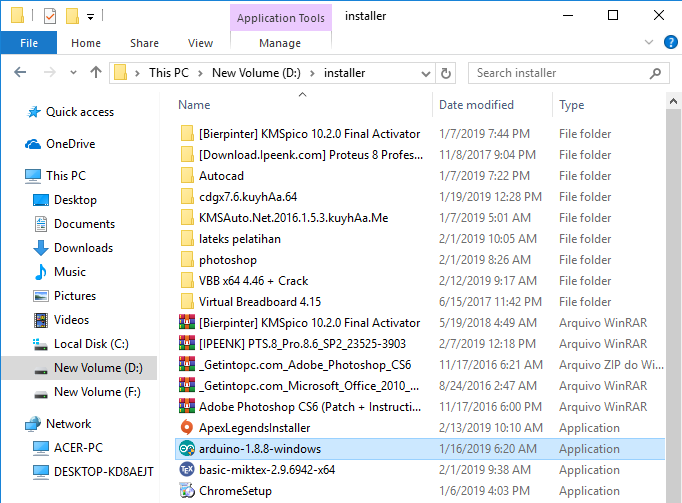
\includegraphics[width=.75\textwidth]{figures/IDE/installer.png}
            \caption{Ini adalah installer}\label{fig:installer}
            \end{figure}
        \item Maka akan tampil seperti gambar \ref{fig:agreement}
            \begin{figure}[!htbp]
            \centering
            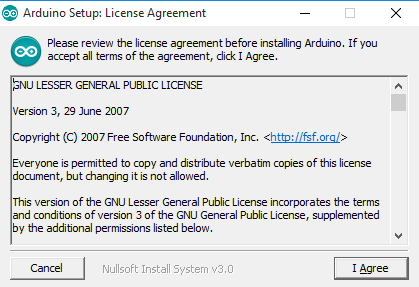
\includegraphics[width=.75\textwidth]{figures/IDE/agreement.png}
            \caption{Ini adalah Halaman Agreement}\label{fig:agreement}
            \end{figure}
        \item Pilih \textbf{Agree} maka akan muncul halaman \textit{Installation Options} seperti pada gambar \ref{fig:option}
            \begin{figure}[!htbp]
            \centering
            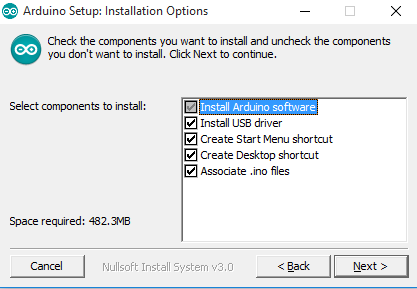
\includegraphics[width=.75\textwidth]{figures/IDE/option.png}
            \caption{Ini adalah Halaman Installation Options}\label{fig:option}
            \end{figure}
        \item Kemudian tekan tombol next, maka akan muncul halaman pemilihan direktori penyimpanan seperti pada gambar \ref{fig:dir}
            \begin{figure}[!htbp]
            \centering
            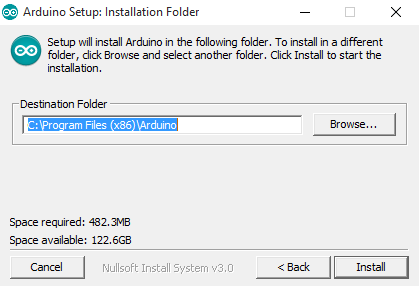
\includegraphics[width=.75\textwidth]{figures/IDE/dir.png}
            \caption{Ini adalah Halaman Pemilihan Direktori}\label{fig:dir}
            \end{figure}
        \item Kemudian tekan tombol install, maka proses installasi dimulai seperti pada gambar \ref{fig:installing}
            \begin{figure}[!htbp]
            \centering
            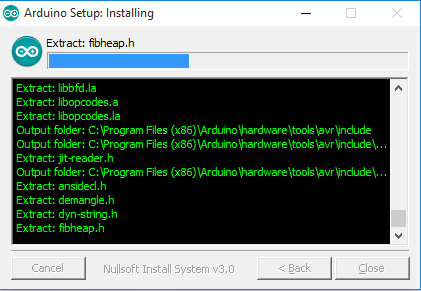
\includegraphics[width=.75\textwidth]{figures/IDE/installing.png}
            \caption{Ini adalah Proses Installasi IDE}\label{fig:installing}
            \end{figure}
        \item Proses installasi selesai, seperti pada gambar \ref{fig:complete}
            \begin{figure}[!htbp]
            \centering
            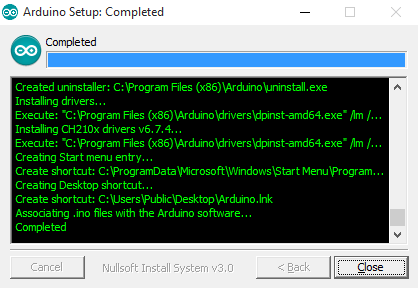
\includegraphics[width=.75\textwidth]{figures/IDE/complete.png}
            \caption{Ini adalah Proses Installasi Telah Selesai}\label{fig:complete}
            \end{figure}
        \end{enumerate}

\chapter{APLIKASI PENDETEKSI BANJIR}
\section{APLIKASI PENDETEKSI BANJIR}

\subsection{KENAPA HARUS APLIKASI INI ?}
\begin{enumerate}
\item Membantu orang apabila terjad bencana banjir
\item Menanggulangi bencana banjir dan menyiapkan warga akanterjadna bencana
\end{enumerate}

\subsection{Alat dan Bahan} 
\begin{enumerate}
\item Arduino
\subitem Arduino adalah pengendali mikro single-board yang bersifat sumber terbuka, diturunkan dari Wiring platform, dirancang untuk memudahkan penggunaan elektronik dalam berbagai bidang
 Pada gambar \ref{labelgambar1} merupakan gambar arduino yang digunakan pada pembuatan alat ini
	\begin{figure}[htbp]
	\centering
	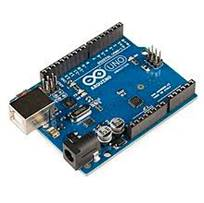
\includegraphics[width=0.5\textwidth]{figures/ALAT_PENDETEKSI_BANJIR/arduino1c}
	\caption{Arduino}
	\label{labelgambar1}
	\end{figure}

\item Bread board
\subitem Breadboard adalah board yang digunakan untuk membuat rangkaian elektronik sementara dengan tujuan uji coba atau prototipe tanpa harus menyolder. Pada gambar \ref{labelgambar2} merupakan gambar Bread Board yang digunakan pada pembuatan alat ini.
	\begin{figure}[htbp]
	\centering
	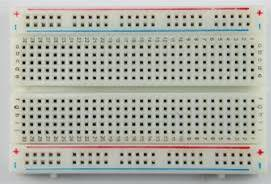
\includegraphics[width=0.5\textwidth]{figures/ALAT_PENDETEKSI_BANJIR/bread_board_1c}
	\caption{Bread Board}
	\label{labelgambar2}
	\end{figure}

\item Kabel jumper 
\subitem kabel penghubung yang biasa digunakan untuk membuat rangkaian sistem atau prototype sistem 	menggunakan arduino dan breadboard. Pada gambar \ref{labelgambar3} merupakan gambar Kabel Jumper yang digunakan pada pembuatan alat ini.
	\begin{figure}[htbp]
	\centering
	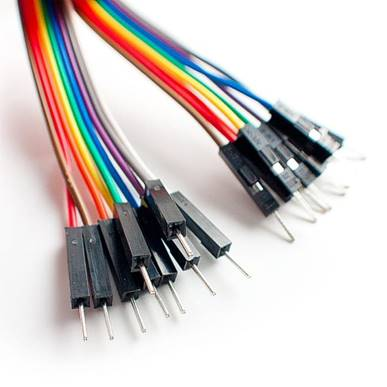
\includegraphics[width=0.5\textwidth]{figures/ALAT_PENDETEKSI_BANJIR/kabel_jumper_1c}
	\caption{Kabel Jumper}
	\label{labelgambar3}
	\end{figure}

\item Pendeteksi sensor ultrasonik
\subitem Sensor yang dapat mendeteksi gelombang ultrasonik, yaitu gelombang suara yang memiliki frekuensi ultrasonik atau frekuensi di atas kisaran frekuensi pendengaran manusia. Pada gambar \ref{labelgambar4} merupakan gambar Pendeteksi Sensor Ultrasonik yang digunakan pada pembuatan alat ini.
	\begin{figure}[htbp]
	\centering
	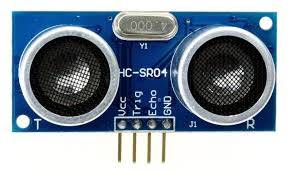
\includegraphics[width=0.5\textwidth]{figures/ALAT_PENDETEKSI_BANJIR/pendeteksi_sensor_ultrasonik_1c}
	\caption{Pendeteksi Sensor Ultrasonik}
	\label{labelgambar4}
	\end{figure}

\item Arduino IDE
\subitem Merupakan aplikasi yang digunakan untuk mengatur program pada arduino. Pada gambar \ref{labelgambar5} merupakan gambar Arduino IDE yang digunakan pada pembuatan alat ini.
	\begin{figure}[htbp]
	\centering
	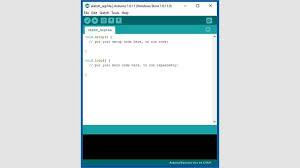
\includegraphics[width=0.5\textwidth]{figures/ALAT_PENDETEKSI_BANJIR/arduino_IDE_1c}
	\caption{Arduino IDE}
	\label{labelgambar5}
	\end{figure}

\item Lampu LED
\subitem Produk diode pancaran cahaya yang disusun menjadi sebuah lampu. Pada gambar \ref{labelgambar6} merupakan gambar Lampu LED yang digunakan pada pembuatan alat ini.
	\begin{figure}[htbp]
	\centering
	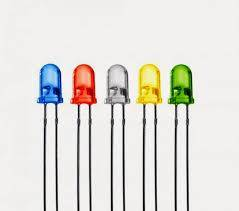
\includegraphics[width=0.5\textwidth]{figures/ALAT_PENDETEKSI_BANJIR/lampu_led_1c}
	\caption{Lampu LED}
	\label{labelgambar6}
	\end{figure}
\end{enumerate}

\subsection{CODE PROGRAMNYA}
\begin{lstlisting}
//defines pins numbers
const int trigPin = 10;
const int echoPin = 11;
//const int buzzer = 12;
const int ledPin= 13;

// defines variables
long duration;
int distance;
int safetyDistance;

void setup() {
  pinMode (trigPin, OUTPUT); // Sets the trigPin as an Output
  pinMode (echoPin, INPUT); // set the echoPin as an Input
 //pinMode(buzzer, OUTPUT);
 pinMode (ledPin, OUTPUT);
 Serial.begin(9600); // Starts the serial communication
}

void loop() {
  // Clears the trigPin
  digitalWrite(trigPin, LOW);
  delayMicroseconds(2);
  // Set the trigPin on HIGH state for 10 micro seconds
  digitalWrite(trigPin, HIGH);
  delayMicroseconds(5);
  digitalWrite(trigPin, LOW);
  // Reads the echoPin, returns the second wave travel time in microseconds
  duration = pulseIn(echoPin, HIGH);
  // Calculating the distance
  distance = duration*0.034/2;
  safetyDistance = distance;
  if (safetyDistance <=10){
    // digitalWrite(buzzer, HIGH);
    digitalWrite(ledPin, HIGH);
  }
  else{
    //digitaWrite (Buzzer, LOW);
    digitalWrite(ledPin, LOW);
  }
 // Prints the distance on the Serial Monitor
 Serial.print("Distance: ");
 Serial.println (distance);
}
\end{lstlisting}

\subsection{BAGAIMANA CARA PASANG NYA?}
\begin{enumerate}
\item Masukan lampu led di port GND dan Port 13
\item Pasang Pendeteksi sensor HC-SR04
\item Sambungkan kabel juper nya dengan urutan port 11 dan 10 di masukan di port echo danport trig
\item Masukan port 5v ke port vcc
\item Masukan port GND ke Port GND
\end{enumerate}

\subsection{Bagaimana Cara Kerja alat nya?}
\begin{enumerate}
\item Sensor diletakan di samping sungai atau di selokan besar
\item Sensor akan berubah warna menjadi warna merah apabila air naik 
\item Sensor akan mendeteksi air pada jarak 10 cm dan akan langsung memberi perigatan banjir 
\end{enumerate}

\subsection{FOTO ALAT PENDETEKSI BANJIR}
Pada gambar \ref{labelgambar7} merupakan gambar alat pendeteksi banjir
\begin{figure}[htbp]
	\centering
	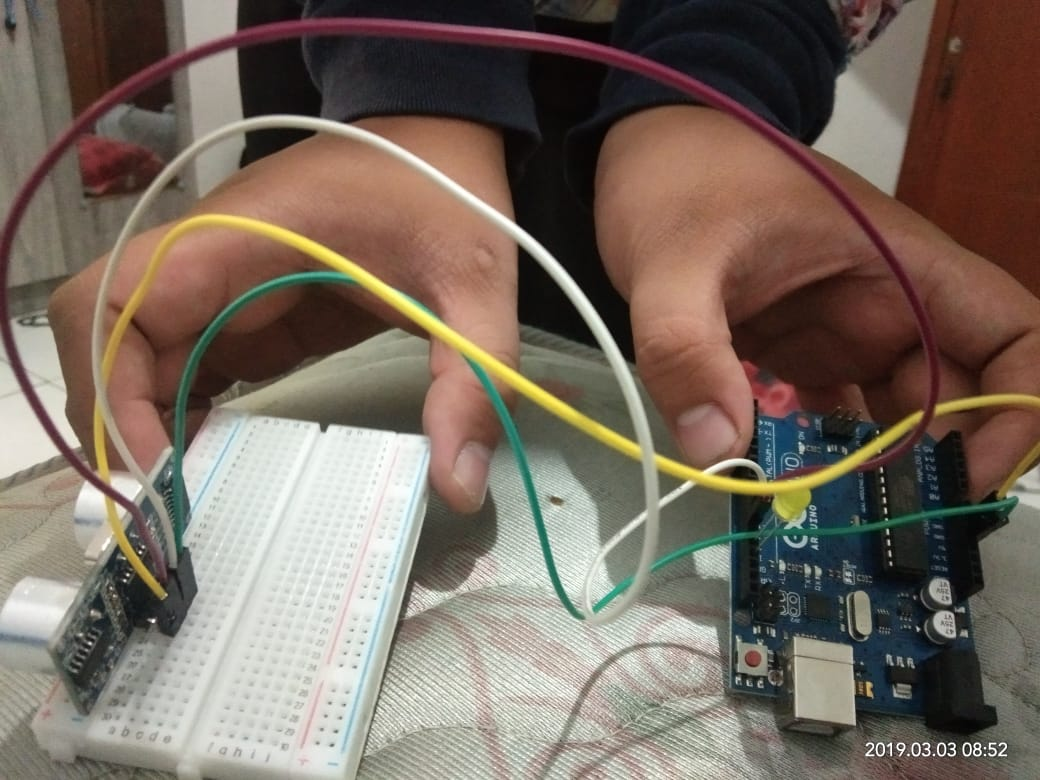
\includegraphics[width=0.5\textwidth]{figures/ALAT_PENDETEKSI_BANJIR/foto_alat_pendeteksi_banjir}
	\caption{Alat Pendeteksi Banjir}
	\label{labelgambar7}
	\end{figure}

\subsection{KESIMPULAN}
Banjir merupakan bencana yang tidak bisa di duga duga oleh manusia dan banjir bisa terjadi dimana mana. Karena itu aplikasi ini dibuat agar orang orang bisa bersiaga menghadapi bencana banjir
 

\bibliographystyle{IEEEtran}
%\def\bibfont{\normalsize}
\bibliography{references}


%%%%%%%%%%%%%%%
%%  The default LaTeX Index
%%  Don't need to add any commands before \begin{document}
\printindex

%%%% Making an index
%%
%% 1. Make index entries, don't leave any spaces so that they
%% will be sorted correctly.
%%
%% \index{term}
%% \index{term!subterm}
%% \index{term!subterm!subsubterm}
%%
%% 2. Run LaTeX several times to produce <filename>.idx
%%
%% 3. On command line, type  makeindx <filename> which
%% will produce <filename>.ind
%%
%% 4. Type \printindex to make the index appear in your book.
%%
%% 5. If you would like to edit <filename>.ind
%% you may do so. See docs.pdf for more information.
%%
%%%%%%%%%%%%%%%%%%%%%%%%%%%%%%

%%%%%%%%%%%%%% Making Multiple Indices %%%%%%%%%%%%%%%%
%% 1.
%% \usepackage{multind}
%% \makeindex{book}
%% \makeindex{authors}
%% \begin{document}
%%
%% 2.
%% % add index terms to your book, ie,
%% \index{book}{A term to go to the topic index}
%% \index{authors}{Put this author in the author index}
%%
%% \index{book}{Cows}
%% \index{book}{Cows!Jersey}
%% \index{book}{Cows!Jersey!Brown}
%%
%% \index{author}{Douglas Adams}
%% \index{author}{Boethius}
%% \index{author}{Mark Twain}
%%
%% 3. On command line type
%% makeindex topic
%% makeindex authors
%%
%% 4.
%% this is a Wiley command to make the indices print:
%% \multiprintindex{book}{Topic index}
%% \multiprintindex{authors}{Author index}

\end{document}

